% Overview figure. Build: pdflatex overview.tex && pdftoppm -png -r 275 -singlefile overview.pdf overview
\documentclass[tikz,border=8pt]{standalone}
\usepackage{paperfig}
\begin{document}
\begin{tikzpicture}[x=1mm,y=1mm]
% ---------- panel backgrounds (explicit so the three top panels align) ----------
\fill[panel, rounded corners=2pt] (0,0) rectangle (44,-60);
\fill[panel, rounded corners=2pt] (50,0) rectangle (154,-60);
\fill[panel, rounded corners=2pt] (160,0) rectangle (216,-60);
\node[paneltitle, anchor=south west, inner xsep=0pt] at (0,0.8) {(a) Task, 100 test flights};
\node[paneltitle, anchor=south west, inner xsep=0pt] at (50,0.8) {(b) Training in simulation};
\node[paneltitle, anchor=south west, inner xsep=0pt] at (160,0.8) {(c) Result in wind};

% ---------- (a) task ----------
\tikzset{taskblock/.style={block, text width=36mm, minimum height=14mm}}
\node[taskblock] (task) at (22,-12) {\blocktitle{Setpoint}{speed, altitude, course\\$V^\ast,\ h^\ast,\ \chi^\ast$}};
\node[taskblock] (wind) at (22,-31) {\blocktitle{Wind}{$\le 5$ m/s, Dryden, noise}};
\node[taskblock] (air)  at (22,-50) {\blocktitle{Airframe}{Aerosonde, PX4 plane}};

% ---------- (b) training ----------
\node[block, text width=30mm, minimum height=50mm] (sim) at (70,-31)
  {\blocktitle{Simulator}{6-DoF, RK4, 100 Hz\\NumPy and C++\\[5pt]C++ matches Python\\to $7{\times}10^{-13}$ over\\7136 steps}};
\node[oursblock, text width=34mm] (actor)  at (131,-11) {\blocktitle{SAC actor}{MLP $64{\times}64$\\PX4 estimates only}};
\node[block, text width=34mm]     (critic) at (131,-33) {\blocktitle{Critics}{MLP $256{\times}256$\\also $\alpha$, $\beta$, true wind}};
\node[ghost, text width=34mm]     (pid)    at (131,-51) {\blocktitle{PID baseline}{same sensors, bank $\le 30^\circ$}};

\foreach \n in {task,wind,air} \draw[flow] (\n.east) -- (\n.east -| sim.west);
\draw[flow] (sim.east |- 0,-8) -- node[lab, above]{$o_t\in\mathbb{R}^{60}$} (actor.west |- 0,-8);
\draw[flow] (actor.west |- 0,-14) -- node[lab, below]{$a_t\in\mathbb{R}^{4}$, 50 Hz} (sim.east |- 0,-14);
\draw[flow] (sim.east |- critic) -- node[lab, above]{$r_t$} (critic.west);
\draw[feedback] (critic.north) -- node[lab, right]{$\nabla_a Q$} (actor.south);
\draw[feedback] (pid.west) -- node[lab, above]{same flights} (pid.west -| sim.east);

% ---------- (c) result ----------
\tikzset{frame/.style={thumb, inner sep=0.5pt, anchor=north west}}
\node[frame] (img) at (162,-3) {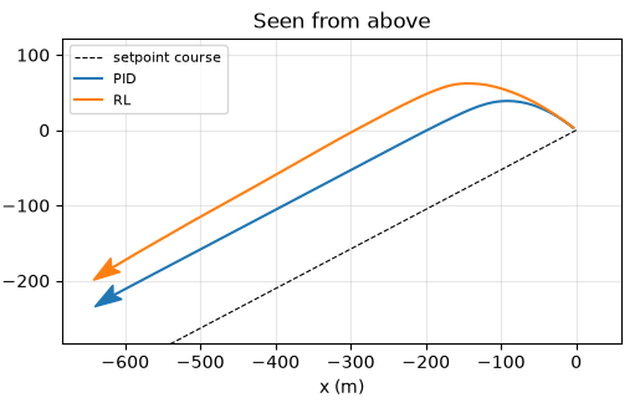
\includegraphics[width=52mm]{ov_topdown.png}};
\draw[flow] (actor.east) -- (actor.east -| img.west);
\node[keynum, anchor=north west, inner xsep=0pt] (k) at ([yshift=-2.5mm]img.south west) {0.59 vs 0.78 m/s};
\node[sub, anchor=north west, align=left, inner xsep=0pt] at ([yshift=-0.5mm]k.south west)
  {airspeed RMS, SAC vs PID\\92 vs 97 of 100 flights complete\\SAC: mean of 3 seeds};

% ---------- (d) thumbnails ----------
\node[paneltitle, anchor=south west, inner xsep=0pt] at (0,-65.5) {(d) Flights in simulation};
\node[frame] (t1) at (0,-66.3)     {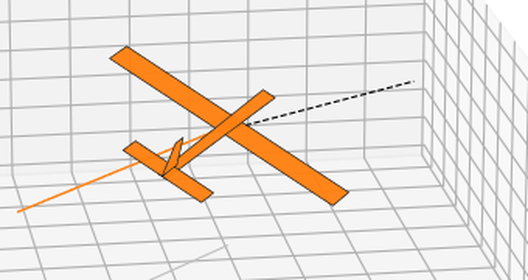
\includegraphics[height=25.5mm]{ov_3d.png}};
\node[frame] (t2) at (56.2,-66.3)  {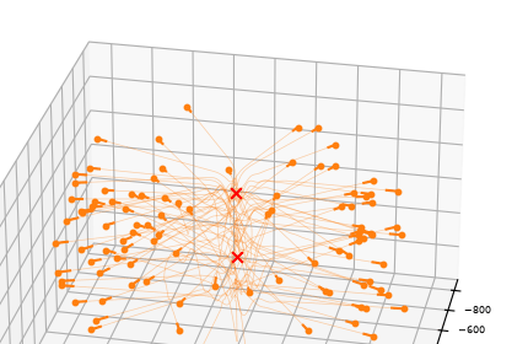
\includegraphics[height=25.5mm]{ov_swarm.png}};
\node[frame] (t3) at (103.4,-66.3) {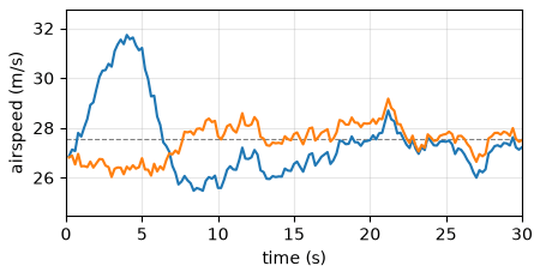
\includegraphics[height=25.5mm]{ov_airspeed.png}};
\foreach \t/\c in {t1/{3D replay, first run}, t2/{100 flights at once, first run}, t3/{Airspeed in wind: SAC orange, PID blue}}
  \node[sub, anchor=north west, inner xsep=0pt] at ([yshift=-1mm]\t.south west) {\c};
\node[anchor=north west, align=left, text width=56mm, inner xsep=0pt, font=\footnotesize] at (160,-66.8)
  {C++, calm air: critic 256 learns,\\critic 64 never learns the course\\[6pt]
   Actor flown by a ROS 2 node\\on PX4 SITL in Gazebo\\[6pt]
   {\color{mid}Simulation only, no real flight}};
\end{tikzpicture}
\end{document}
